\section{The assignment at $k = 2$}
\label{sec:assignment}

\subsection{The original run}

The original run scaled each feature to $[0, 1]$ on all rows, drew one Eq.~3 and one Eq.~4 matrix per data set with seed 42, projected to $k = 2$, made one stratified 70/30 split, and trained four SVMs with default settings. Table~\ref{tab:original} gives the test accuracy. The report took the best of the four kernels on the test set for each distribution. By that rule, Eq.~4 minus Eq.~3 is \N{o:iris:delta} points on Iris, \N{o:breast_cancer:delta} on Breast Cancer, \N{o:wine:delta} on Wine, \N{o:seeds:delta} on Seeds, and \N{o:glass:delta} on Glass. Test sets are small (\N{z:n_test:iris} rows for Iris and \N{z:n_test:glass} for Glass), so one row moves the accuracy by \N{z:row_pts:iris} points on Iris and \N{z:row_pts:glass} on Glass.

\begin{table*}[t]
\caption{Test accuracy (\%, plain accuracy for every data set) of the original run: one matrix per distribution, one split, default SVMs, $k = 2$. Lin.: linear; P2, P3: polynomial of degree 2 and 3.}
\label{tab:original}
\centering
\footnotesize
\setlength{\tabcolsep}{4pt}
\begin{tabular}{@{}lcccccccc@{}}
\toprule
 & \multicolumn{4}{c}{Eq. 3} & \multicolumn{4}{c}{Eq. 4} \\
\cmidrule(lr){2-5}\cmidrule(lr){6-9}
Data set & Lin. & P2 & P3 & RBF & Lin. & P2 & P3 & RBF \\
\midrule
Iris & 80.0 & 84.4 & 84.4 & 80.0 & 68.9 & 68.9 & 68.9 & 68.9 \\
Breast Cancer & 82.5 & 80.1 & 77.8 & 81.3 & 84.2 & 83.6 & 83.6 & 83.6 \\
Wine & 64.8 & 61.1 & 57.4 & 55.6 & 66.7 & 68.5 & 64.8 & 70.4 \\
Seeds & 79.4 & 84.1 & 84.1 & 82.5 & 90.5 & 85.7 & 85.7 & 92.1 \\
Glass & 38.5 & 49.2 & 46.2 & 56.9 & 52.3 & 44.6 & 46.2 & 55.4 \\
\bottomrule
\end{tabular}

\end{table*}

\subsection{The Iris tie}

On Iris, Eq.~4 gave \N{o:iris:eq4:linear}\% under all four kernels. The seed-42 Eq.~4 matrix has zero entries in both petal rows, so the projection used only sepal length and sepal width, one in each column. The four kernels predict the same \N{z:n_test:iris} test labels, but they are different models: their training accuracies differ. An Eq.~4 matrix zeroes both petal rows with probability $(2/3)^4 = \N{z:theory_both_iris}\%$, and most such matrices also lose a dimension; this one kept two, so it was not a collapse.

\subsection{The same pipeline over 100 draws}

To see how far one draw can mislead, the unchanged pipeline was repeated for seeds 0 to 99, which include 42. Table~\ref{tab:replication} and Fig.~\ref{fig:replication} give the result. The report's Eq.~4 draw on Seeds, \N{rep:seeds:best_kernel_acc_eq4:report_seed42}\%, is above \N{rep:seeds:best_kernel_acc_eq4:draws_lower} of the other 99 draws, ties \N{rep:seeds:best_kernel_acc_eq4:draws_equal_excl_42}, and is below \N{rep:seeds:best_kernel_acc_eq4:draws_higher} (median \N{rep:seeds:best_kernel_acc_eq4:median}\%). The paired difference between Eq.~4 and Eq.~3 is negative on Iris, \N{rep:iris:best_eq4_minus_best_eq3} points with a 95\% interval of [\N{rep:iris:best_eq4_minus_best_eq3:ci_low}, \N{rep:iris:best_eq4_minus_best_eq3:ci_high}], and positive on Seeds, \N{rep:seeds:best_eq4_minus_best_eq3} [\N{rep:seeds:best_eq4_minus_best_eq3:ci_low}, \N{rep:seeds:best_eq4_minus_best_eq3:ci_high}]. The other three intervals include zero. These intervals are not adjusted across the five data sets, and they all use the report's one split, so only the matrices vary. The report also chose each kernel on the test set. ``Eq.~4 outperforms Eq.~3 on three of five data sets'' was not a rare draw: \N{rep3:ge3} of the 100 draws put Eq.~4 strictly ahead on three or more data sets. What one draw cannot show is a consistent difference. Only on Seeds and Iris does the interval of the mean difference exclude zero (unadjusted), favoring Eq.~4 on Seeds and Eq.~3 on Iris, and in the tuned study of Section~\ref{sec:classification}, which also changes the pipeline (it scales on the training rows only, standardizes after projecting, tunes each kernel and picks one by inner cross-validation, and draws a new split for each draw), the Seeds difference at $k = 2$ is \N{pd:seeds:2:eq4:eq3} points [\N{pd:seeds:2:eq4:eq3:lo}, \N{pd:seeds:2:eq4:eq3:hi}].

\begin{table*}[t]
\caption{The original pipeline over 100 draws of the matrices (seeds 0 to 99), for Eq.~3 and Eq.~4: mean test accuracy (\%, plain accuracy for every data set) of the best kernel, chosen on the test set as in the report, with a 95\% bootstrap interval; the report's draw; and the paired difference.}
\label{tab:replication}
\centering
\footnotesize
\setlength{\tabcolsep}{3pt}
\begin{tabular}{@{}lcccc@{}}
\toprule
Data set & Eq. 3, best kernel & Eq. 4, best kernel & Report draw (Eq. 3 / Eq. 4) & Eq. 4 $-$ Eq. 3 (points) \\
\midrule
Iris & 85.4 [83.1, 87.4] & 79.2 [75.9, 82.4] & 84.4 / 68.9 & $-$6.2 [$-$10.1, $-$2.4] \\
Breast Cancer & 84.9 [83.3, 86.4] & 84.5 [82.9, 86.0] & 82.5 / 84.2 & $-$0.4 [$-$2.5, 1.7] \\
Wine & 71.4 [69.3, 73.6] & 73.4 [71.3, 75.5] & 64.8 / 70.4 & 2.0 [$-$0.8, 4.7] \\
Seeds & 76.3 [74.5, 77.9] & 79.3 [77.3, 81.2] & 84.1 / 92.1 & 3.1 [0.5, 5.6] \\
Glass & 56.3 [54.9, 57.6] & 54.2 [52.8, 55.6] & 56.9 / 55.4 & $-$2.0 [$-$4.2, 0.1] \\
\bottomrule
\end{tabular}

\end{table*}

\begin{figure}[t]
\centering
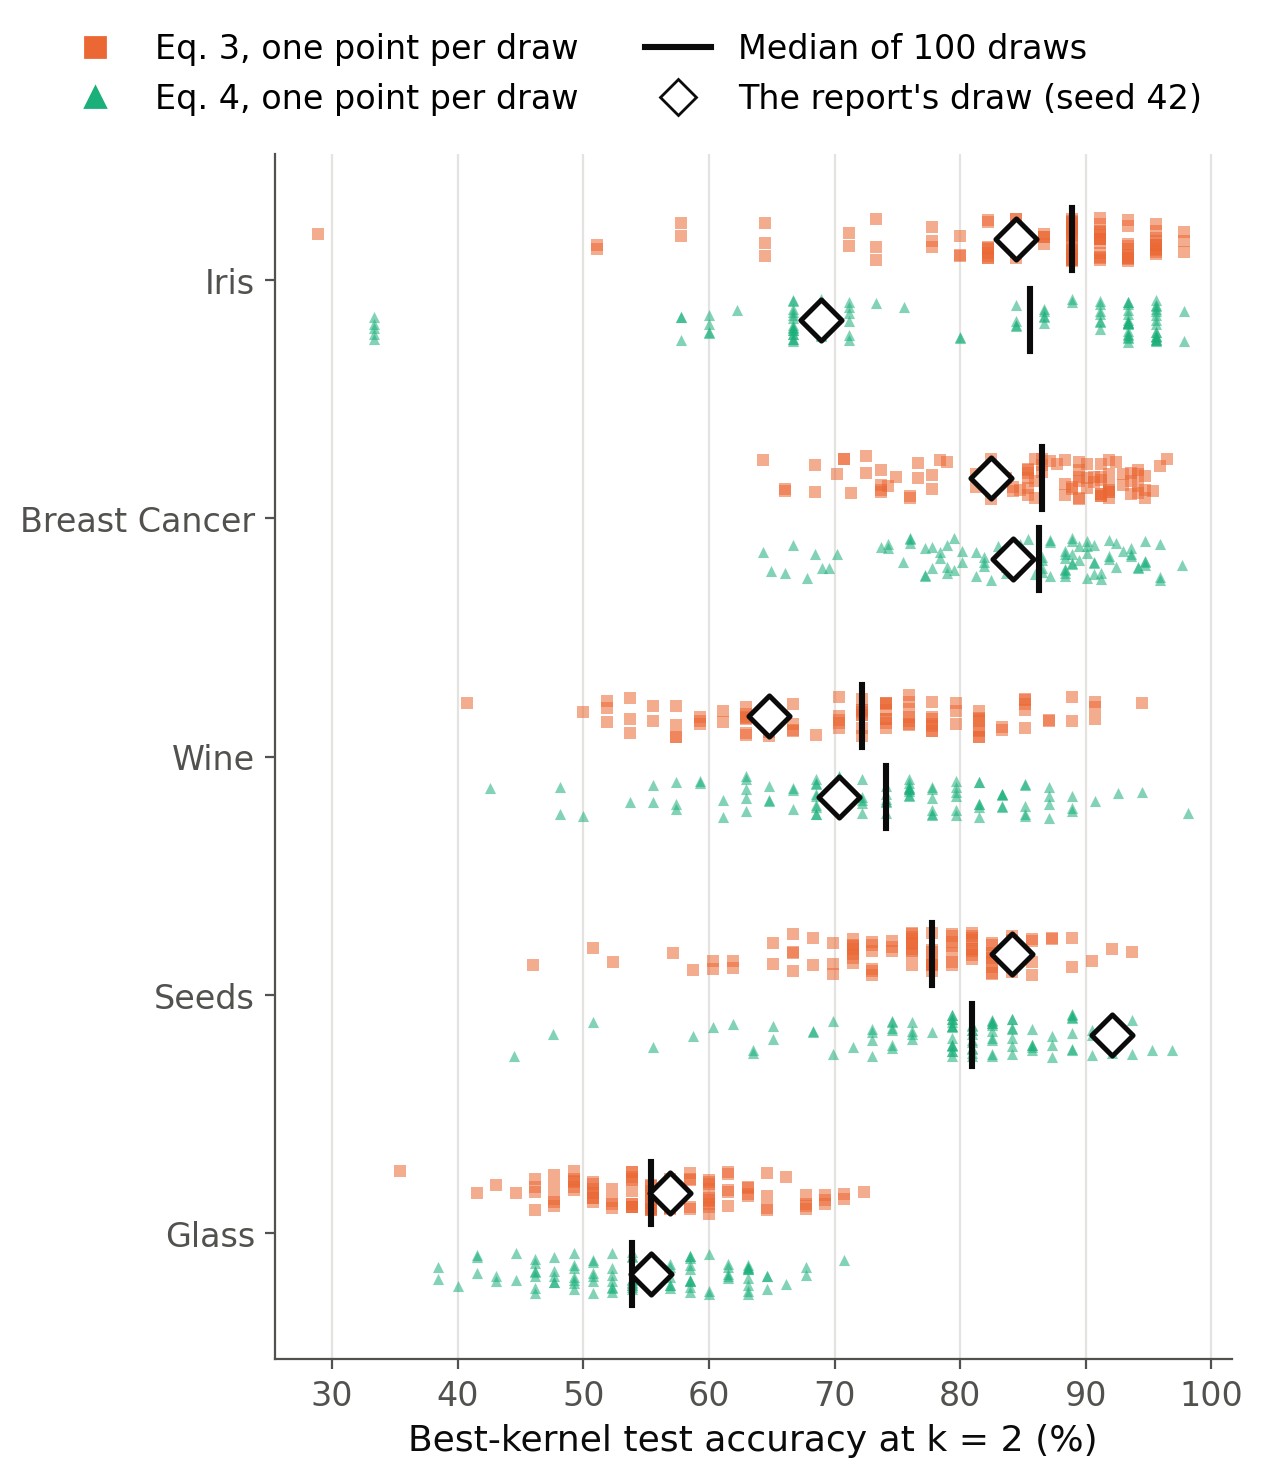
\includegraphics[width=\columnwidth]{../study/figures/fig7_original_pipeline_100_draws.png}
\caption{Best-kernel test accuracy at $k = 2$ for Eq.~3 (squares) and Eq.~4 (triangles), one point per draw over 100 draws, with each median and the report's draw (seed 42). The best kernel is chosen on the test set, as in the report.}
\label{fig:replication}
\end{figure}

\subsection{Distortion at $k = 2$}

The report summarized distortion by the smallest and largest ratio of projected to original distances over all pairs, and an $\varepsilon$ computed from them. At $k = 2$, that $\varepsilon$ runs from \N{z:eps_min} to \N{z:eps_max}. With $\varepsilon$ at or near 1, the lower Johnson--Lindenstrauss inequality is vacuous or nearly so, so these values cannot say how well the lemma held. The mean squared-distance ratio, which is unbiased, is the better summary (Section~\ref{sec:distortion}).
